\documentclass{article}

%\usepackage{pgf}
\usepackage{tikz}
\usetikzlibrary{arrows,automata}
\title{Finite Automata in \LaTeX{} with {\tt tikz}}
\author{Geoffrey Matthews}
\begin{document}
\maketitle

\section{Illustrations from the textbook}
Here is the figure from page 29:

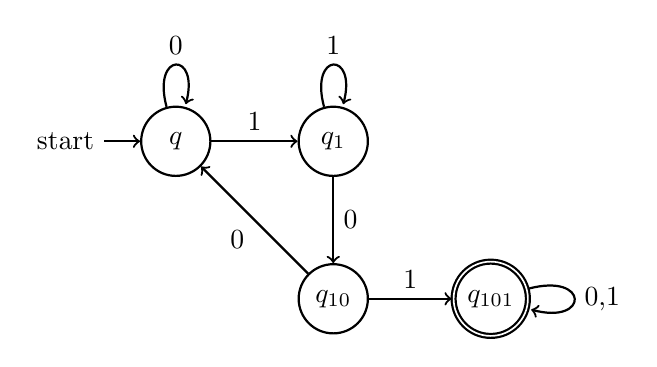
\begin{tikzpicture}[->,auto,node distance=2cm,thick]

  \node[initial,state]     (0)               {$q$};
  \node[state]             (1) [right of=0]  {$q_1$};
  \node[state]            (10) [below of=1]  {$q_{10}$};
  \node[state,accepting] (101) [right of=10] {$q_{101}$};

  \path (0)   edge [loop above] node {0} (0)
              edge              node {1} (1)
        (1)   edge [loop above] node {1} (1)
              edge              node {0} (10)
        (10)  edge              node {0} (0)
              edge              node {1} (101)
        (101) edge [loop right] node {0,1} (101);
\end{tikzpicture}

Here is the figure from page 30, with some different arrows:

%\begin{tikzpicture}[->,>=stealth',shorten >=1pt,auto,node distance=3cm,thick]
\begin{tikzpicture}[->,>=stealth',auto,node distance=3cm,thick]

  \node[initial,state]   (000)                    {$q_{000}$};
  \node[state,accepting] (100) [right of=000]     {$q_{100}$};
  \node[state]           (010) [right of=100]     {$q_{010}$};
  \node[state,accepting] (110) [right of=010]     {$q_{110}$};
  \node[state]           (001) [below of=000]     {$q_{001}$};
  \node[state,accepting] (101) [right of=001]     {$q_{101}$};
  \node[state]           (011) [right of=101]     {$q_{011}$};
  \node[state,accepting] (111) [right of=011]     {$q_{111}$};

  \path (000) edge [loop above]     node         {0} (000)
              edge                  node         {1} (001)
        (100) edge                  node         {0} (000)
              edge                  node         {1} (001)
        (010) edge                  node         {0} (100)
              edge [out=-130,in=40] node [right] {1} (101)
        (110) edge [bend right]     node [above] {0} (100)
              edge                  node         {1} (101)
        (001) edge                  node         {0} (010)
              edge [bend right]     node [below] {1} (011)
        (101) edge [out=50,in=-140] node [left]  {0} (010)
              edge                  node         {1} (011)
        (011) edge                  node         {0} (110)
              edge                  node         {1} (111)
        (111) edge                  node         {0} (110)
              edge [loop below]     node         {1} (111);

\end{tikzpicture}

Bend right and bend left automatically curve the arrows.
In the above picture, the arrows between 010 and 101 had to be
squeezed in tightly, hence the specification of in and out angles.

The same picture done with a matrix layout for the nodes:

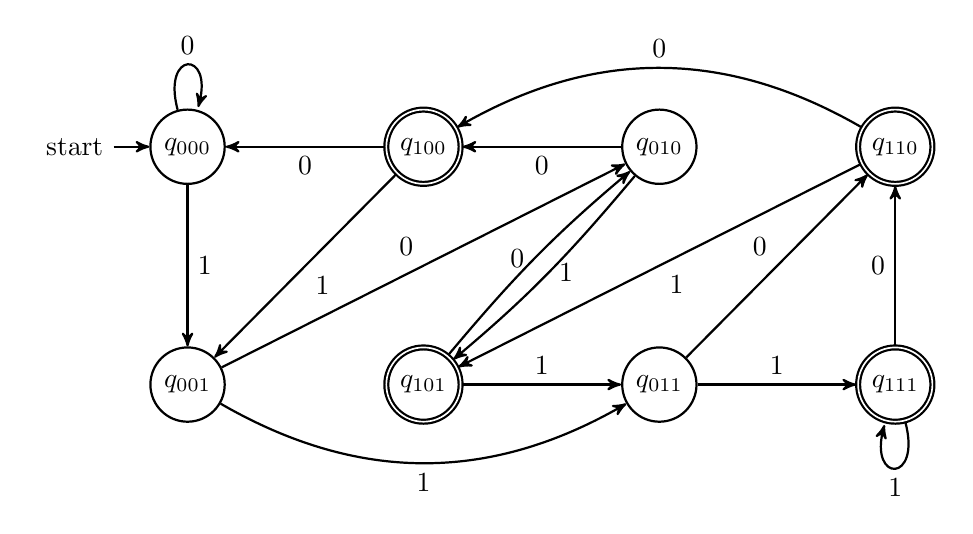
\begin{tikzpicture}[->,>=stealth',auto,thick]
\matrix[row sep = 2cm, column sep=2cm]{
  \node[initial,state]   (000)    {$q_{000}$}; &
  \node[state,accepting] (100)    {$q_{100}$}; &
  \node[state]           (010)    {$q_{010}$}; &
  \node[state,accepting] (110)    {$q_{110}$}; \\
  \node[state]           (001)    {$q_{001}$}; &
  \node[state,accepting] (101)    {$q_{101}$}; &
  \node[state]           (011)    {$q_{011}$}; &
  \node[state,accepting] (111)    {$q_{111}$}; \\
  };

  \path (000) edge [loop above]     node         {0} (000)
              edge                  node         {1} (001)
        (100) edge                  node         {0} (000)
              edge                  node         {1} (001)
        (010) edge                  node         {0} (100)
              edge [out=-130,in=40] node [right] {1} (101)
        (110) edge [bend right]     node [above] {0} (100)
              edge                  node         {1} (101)
        (001) edge                  node         {0} (010)
              edge [bend right]     node [below] {1} (011)
        (101) edge [out=50,in=-140] node [left]  {0} (010)
              edge                  node         {1} (011)
        (011) edge                  node         {0} (110)
              edge                  node         {1} (111)
        (111) edge                  node         {0} (110)
              edge [loop below]     node         {1} (111);

\end{tikzpicture}

\section{Martin Thoma examples}

Examples on a web page I found:

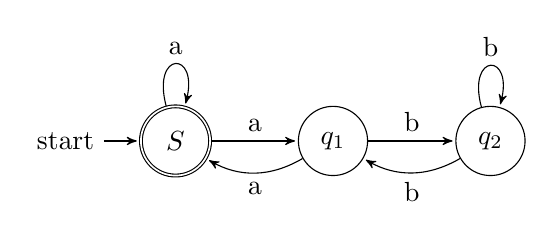
\begin{tikzpicture}[>=stealth',shorten >=1pt,auto,node distance=2cm]
  \node[initial,state,accepting] (S)      {$S$};
  \node[state]         (q1) [right of=S]  {$q_1$};
  \node[state]         (q2) [right of=q1] {$q_2$};


  \path[->] (S)  edge [loop above] node {a} (S)
             edge              node {a} (q1)
        (q1) edge [bend left]  node {a} (S)
             edge              node {b} (q2)
        (q2) edge [loop above] node {b} (q2)
             edge [bend left]  node {b} (q1);
\end{tikzpicture}


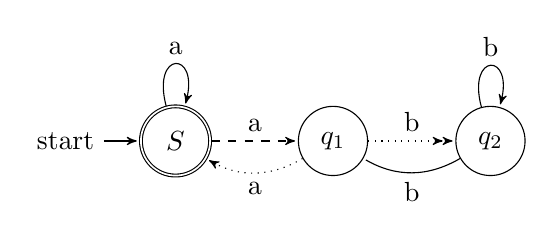
\begin{tikzpicture}[>=stealth',shorten >=1pt,auto,node distance=2cm]
  \node[initial,state,accepting] (S)      {$S$};
  \node[state]         (q1) [right of=S]  {$q_1$};
  \node[state]         (q2) [right of=q1] {$q_2$};

  \path[->]          (S)  edge [loop above] node {a} (S);
  \path[->, dashed]  (S)  edge              node {a} (q1);
  \path[->, dotted]  (q1) edge [bend left]  node {a} (S);
  \path[->>, dotted] (q1) edge             node {b} (q2);
  \path              (q2) edge [loop above] node {b} (q2)
             edge [bend left]  node {b} (q1);
\end{tikzpicture}

\section{Example from the PGF/TikZ manual}

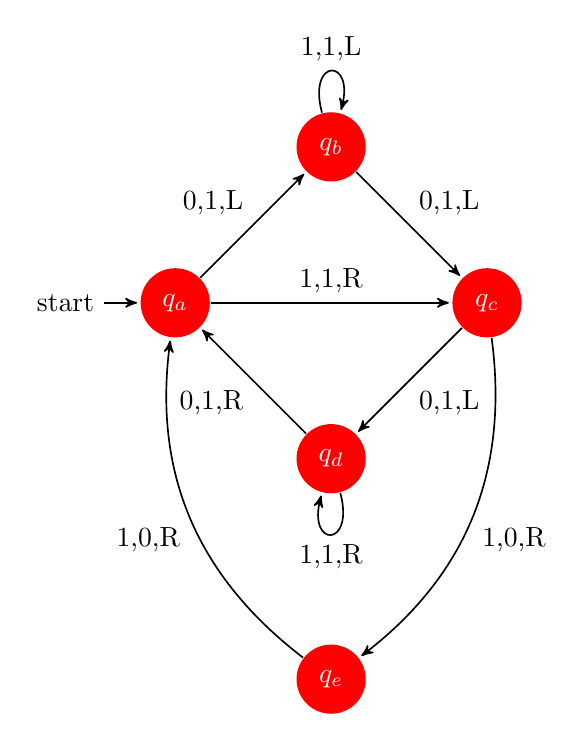
\begin{tikzpicture}[->,>=stealth',shorten >=1pt,auto,node distance=2.8cm,
                    semithick]
  \tikzstyle{every state}=[fill=red,draw=none,text=white]

  \node[initial,state] (A)                    {$q_a$};
  \node[state]         (B) [above right of=A] {$q_b$};
  \node[state]         (D) [below right of=A] {$q_d$};
  \node[state]         (C) [below right of=B] {$q_c$};
  \node[state]         (E) [below of=D]       {$q_e$};

  \path (A) edge              node {0,1,L} (B)
            edge              node {1,1,R} (C)
        (B) edge [loop above] node {1,1,L} (B)
            edge              node {0,1,L} (C)
        (C) edge              node {0,1,L} (D)
            edge [bend left]  node {1,0,R} (E)
        (D) edge [loop below] node {1,1,R} (D)
            edge              node {0,1,R} (A)
        (E) edge [bend left]  node {1,0,R} (A);
\end{tikzpicture}




\end{document}
